% sample.tex
\documentclass[pdf,swa,slideBW,nocolorBG,nototal]{prosper}
% \usepackage[dvips]{geometry}
%\usepackage{ngerman}
\usepackage{graphicx}
\usepackage{wrapfig, rotating}
\usepackage[T1]{fontenc}

\title{Tracing Object Lifetime}
\author{Christoph Neijenhuis, Tobias Mohr, Tim Felgentreff}
%\email{\{christoph.neijenhuis, tobias.mohr, fim.felgentreff\}@student.hpi.uni-potsdam.de}
\institution{
        Agile Software Development \\
        Hasso-Plattner-Institut \\
        Universit�t Potsdam\\
        SS 2011
}
\foot{Agile Software Development 2011 | Felgentreff, Mohr, Neijenhuis | \today }

\begin{document}

\maketitle

\begin{slide}{Demo}
  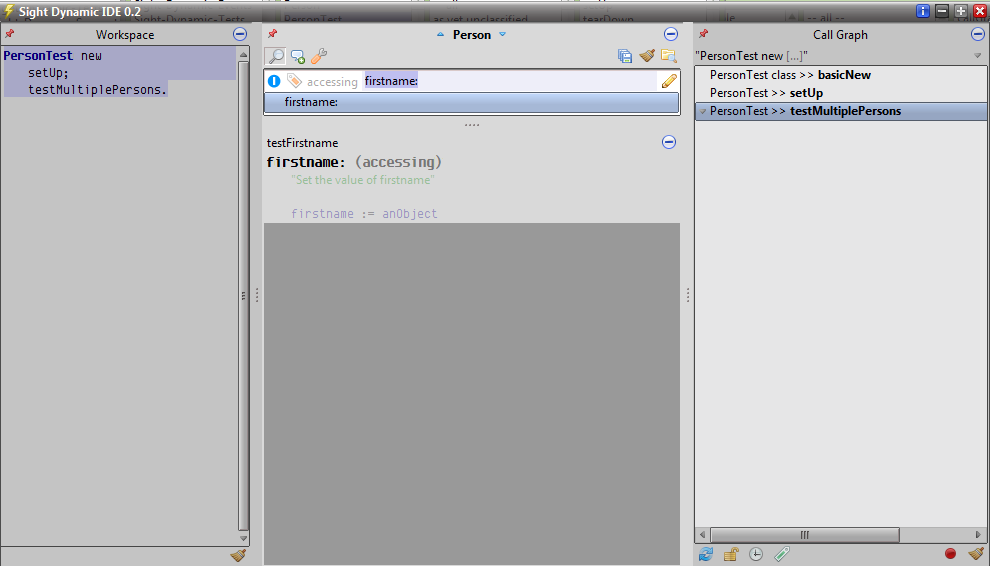
\includegraphics[width=\linewidth]{pics/sdide_intro}
\end{slide}

\begin{slide}{Agenda}
  \begin{itemize}
  \item Come again (Previously, on Agile-SD-1)
  \item Improved Tests (Return of Readability)
  \item Developer Stories (A New Scope)
  \item Different Visions (Research Strikes Back)
  \end{itemize}
\end{slide}

\overlays{2}{%
\begin{slide}{Previously\ldots}
  \begin{itemize}
  \item Management with ``offline'' story cards
  \item Bi-weekly meetings
  \item Weekly story choices \& estimates
  \end{itemize}
  \fromSlide{2}{%
    {\bf Critique}
    \begin{itemize}
    \item Insufficient traceability
    \item Somewhat fragile testing \& continuous testing infrastructure
    \item General lack of motivating vision
    \end{itemize}}
\end{slide}
}

\begin{slide}{Tests - First Contact}
  \parbox[t]{0.6\textwidth}{%
    \vspace*{2.5cm}
    \hspace*{7cm}
    \begin{rotate}{353}
      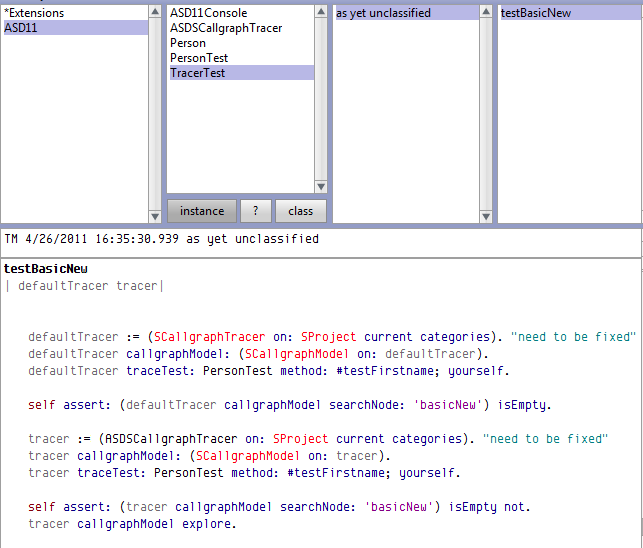
\includegraphics[width=0.7\linewidth]{pics/workspace_test}
    \end{rotate}}
  \begin{itemize}
  \item Hard to ``test-ahead''
  \item Tests developed in parallel with implementation
  \item Code-first $\Rightarrow$ hard to test code
  \item First test were hard to read
  \end{itemize}
\end{slide}

\begin{slide}{Tests - Ensuring Traceability}
  \parbox[t]{0.6\textwidth}{%
    \vspace*{2.5cm}
    \hspace*{4cm}
    \begin{rotate}{353}
      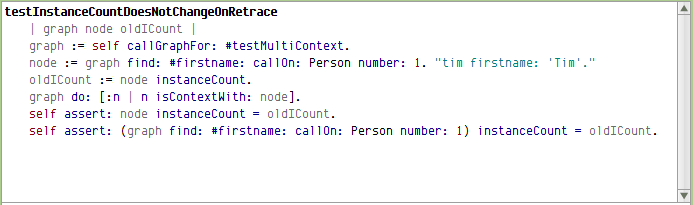
\includegraphics[width=1.3\linewidth]{pics/good_test}
    \end{rotate}}
  \vspace*{1.5cm}
  \begin{itemize}
  \item Forcing ourselves to write {\sc X} tests for each story card
    \begin{itemize}
    \item More readable tests
    \item More consistent {\sc API}
    \item Better estimates
    \end{itemize}
  \end{itemize}
\end{slide}

\begin{slide}{Tests - Run, Code, Run}
  \centering
  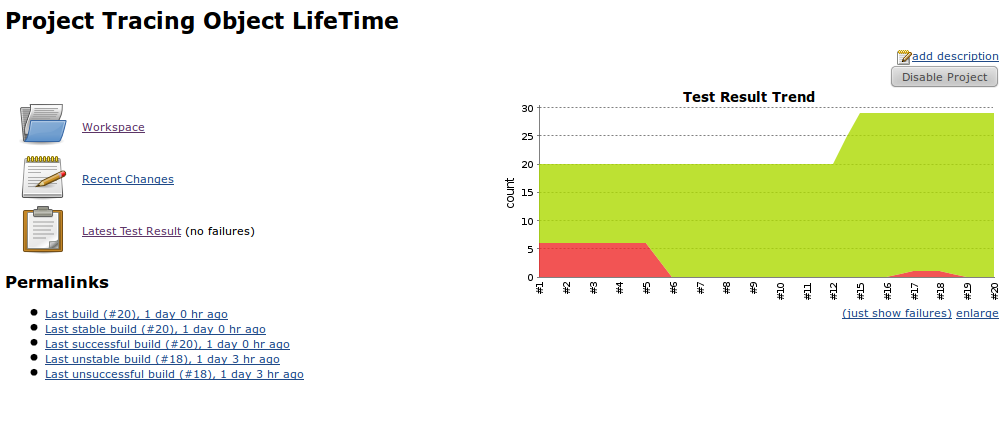
\includegraphics[width=\linewidth]{pics/ci}
  \begin{itemize}
  \item Continuous Integration
  \end{itemize}
\end{slide}

\overlays{2}{%
\begin{slide}{User Stories - There are never enough}
  \begin{itemize}
  \item Customer is constrained
    \begin{itemize}
    \item Has different projects
    \item Doesn't have time to think up stories every other week
    \item Needs old stories for context
    \end{itemize}
  \fromSlide{2}{%
  \item Building a backlog is important
    \begin{itemize}
    \item Clearer heading
    \item More choice = more freedom
    \end{itemize}}
  \end{itemize}
\end{slide}}

\begin{slide}{User Stories - {\sc DIY}}
  \begin{itemize}
  \item ``Make it your project''
    \begin{itemize}
    \item We tried to analyze existing projects
    \item We came up with stories of our own
    \end{itemize}
  \item Start to think
    \begin{itemize}
    \item The customer wants a solution, not a better description of
      the problem
    \item Come up with (mutually exclusive) alternatives
    \end{itemize}
  \end{itemize}
\end{slide}

\overlays{3}{%
\begin{slide}{Different Visions - It's about scope}
  \fromSlide{2}{%
  {\bf Customer}
  \begin{itemize}
  \item Wants as much as possible
  \item Avoids restricting the project scope
  \item Expects steady progress
  \end{itemize}}
  \fromSlide{3}{%
  {\bf Developer}
  \begin{itemize}
  \item Wants small, clean, isolated task modules
  \item Tries to narrow down desired scope
  \item Motivates himself on steady progress
  \end{itemize}}
\end{slide}}

\overlays{3}{%
\begin{slide}{Different Visions - Force your customer}
  \begin{itemize}
  \item Developer-supplied stories revealed different visions
  \item Mockups helped talking about ideas
  \fromSlide{2}{%
    \hspace*{1cm}
    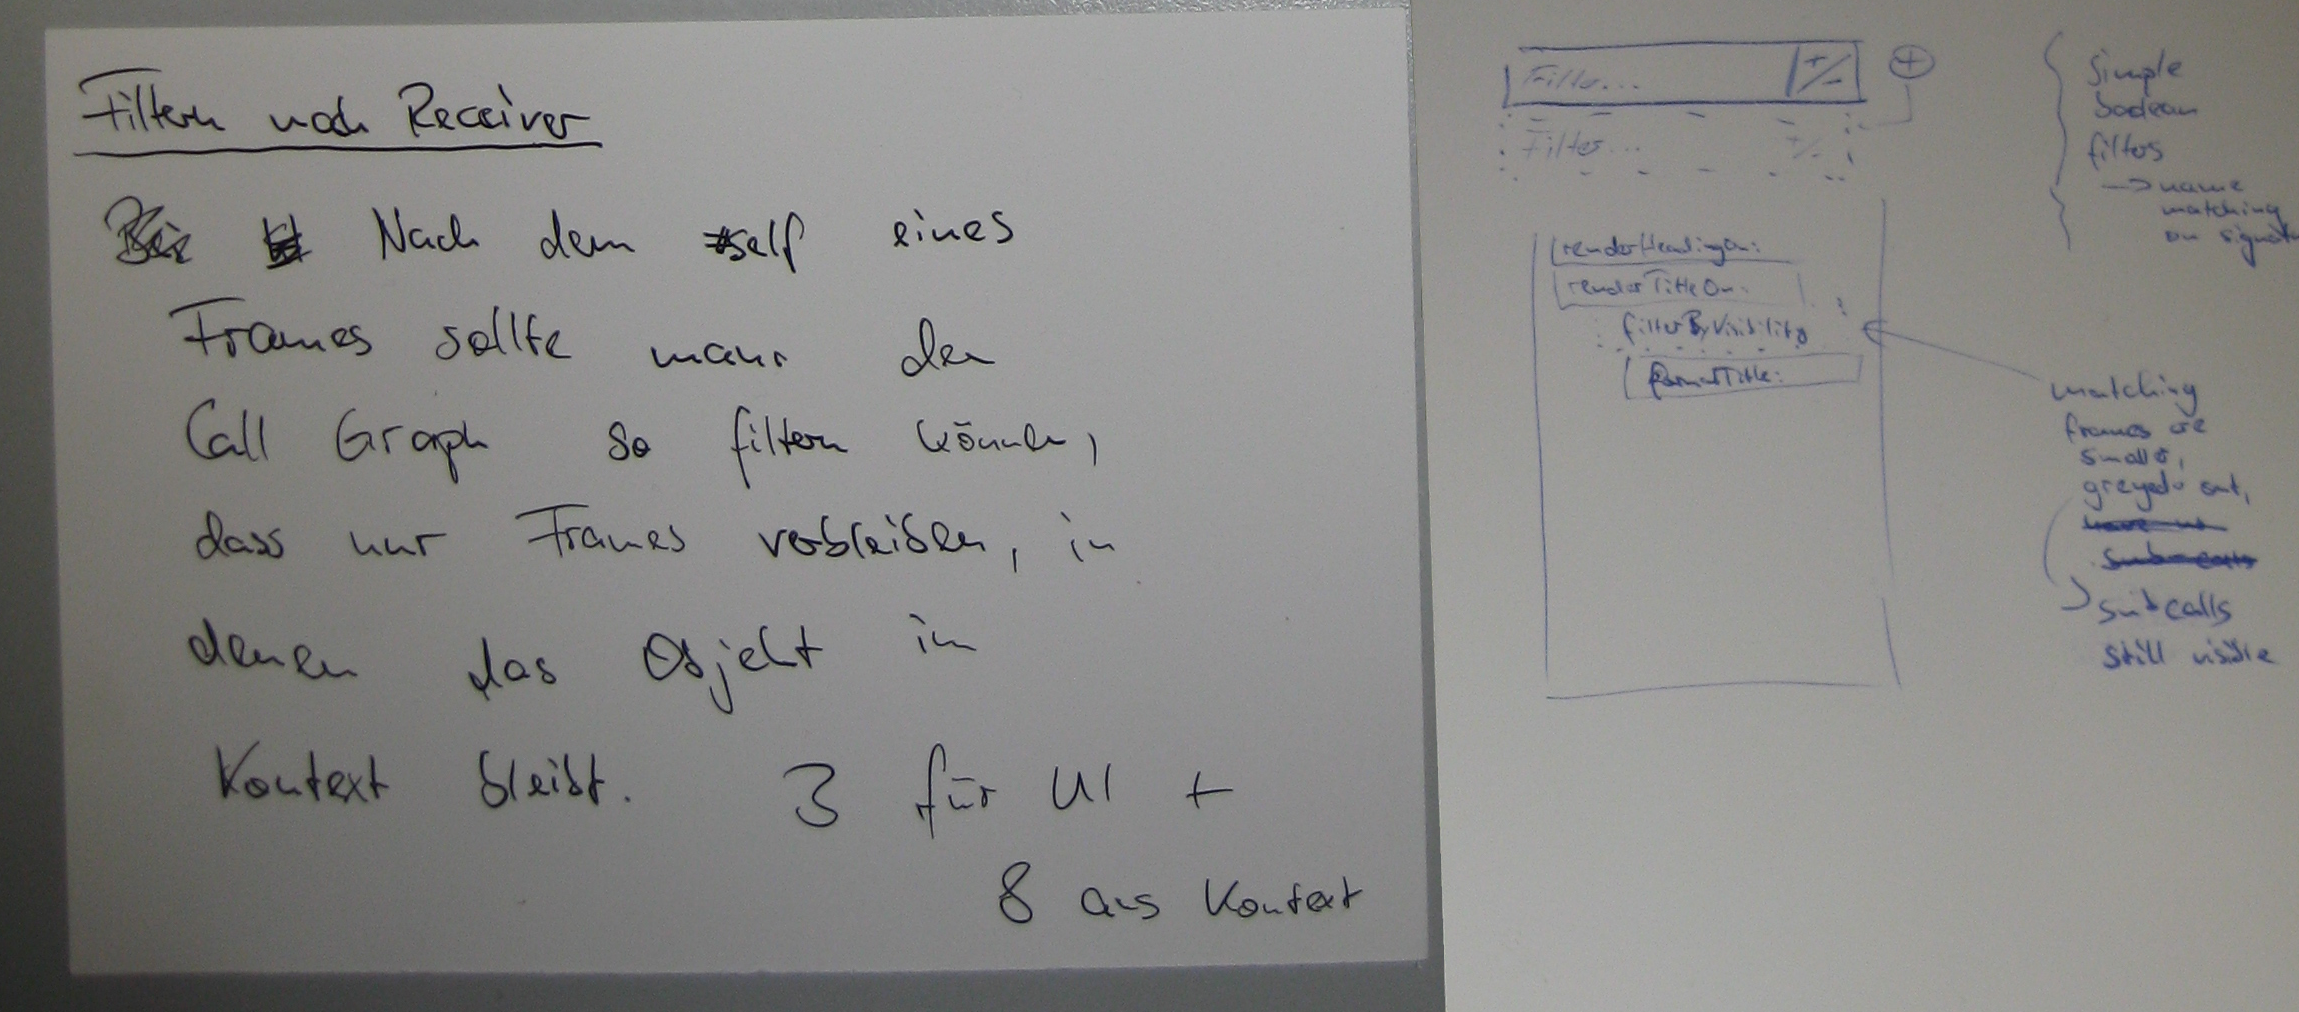
\includegraphics[width=0.7\linewidth]{pics/mockups}
  }
  \item The customer was forced to restrict scope
  \fromSlide{3}{%
  \item \Large{Great Success!}}
  \end{itemize}
\end{slide}}

\begin{slide}{Conclusions}
  \begin{itemize}
  \item We're understanding our customer's problem better
  \item Still trying to figure out how to track non-story work
    {\footnotesize (like this presentation)}
  \item We've gotten good at ``test first'' --- just needed to sit
    down and do-it\texttrademark
  \end{itemize}
\end{slide}

\begin{slide}{}
  \nocite{*}
  \bibliographystyle{splncs}
  {\small \bibliography{swt.bib}}
\end{slide}

\end{document}
